\documentclass[tikz,border=7pt]{standalone}
\usepackage{amsmath}
\usetikzlibrary{arrows.meta,positioning}
\tikzset{
  wfstep/.style={draw,rectangle,rounded corners=2pt,minimum width=36mm,minimum height=18mm,align=center},
  arr/.style={-{Latex[length=2.2mm]},thick}
}
\begin{document}
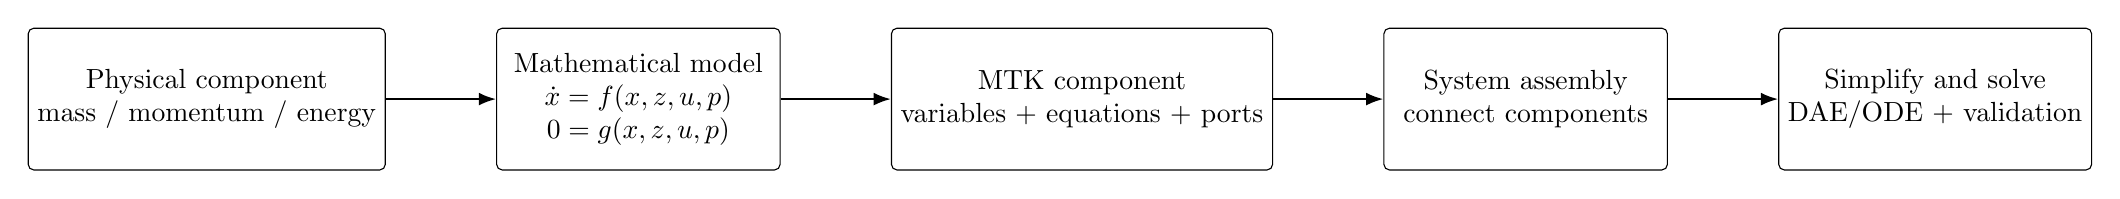
\begin{tikzpicture}[node distance=14mm]
\node[wfstep] (physics) {Physical component\\mass / momentum / energy};
\node[wfstep,right=of physics] (math) {Mathematical model\\$\dot x=f(x,z,u,p)$\\$0=g(x,z,u,p)$};
\node[wfstep,right=of math] (mtk) {MTK component\\variables + equations + ports};
\node[wfstep,right=of mtk] (assembly) {System assembly\\connect components};
\node[wfstep,right=of assembly] (solve) {Simplify and solve\\DAE/ODE + validation};
\draw[arr] (physics) -- (math);
\draw[arr] (math) -- (mtk);
\draw[arr] (mtk) -- (assembly);
\draw[arr] (assembly) -- (solve);
\end{tikzpicture}
\end{document}
